\section{Własny zbiór danych}

W ramach pracy przygotowałem własny zbiór próbek pisma odręcznego. Zbiór powstał na potrzeby badań nad rozpoznawaniem tekstu pisanego ręcznie. Szczególnie ważne były próbki pisma osób z dysgrafią. Chciałem jednak porównać wyniki także z pismem osób bez zadeklarowanych trudności.

Dane zbierałem w szkołach w Augustowie oraz w jednej szkole w Gdańsku. Uczestnicy wypełniali papierowe formularze. Udział w badaniu był dobrowolny i anonimowy. Formularz nie zawierał imienia, nazwiska ani innych danych, które pozwalałyby łatwo zidentyfikować uczestnika.

Każdy uczestnik podawał podstawowe informacje o sobie. Były to: płeć, rok urodzenia oraz informacja o trudnościach w pisaniu. W formularzu można było zaznaczyć brak trudności, dysgrafię albo inne trudności. Do tej ostatniej grupy trafiły między innymi osoby z dysleksją lub dysortografią. Informacje te traktuję jako deklaracje uczestników. Nie są one niezależną diagnozą medyczną wykonaną w ramach tej pracy.

Przygotowałem trzy wersje formularza: zestaw A, zestaw B oraz zestaw C. Każdy zestaw zawierał osiem tekstów do przepisania. Uczestnik przepisywał każdy tekst w osobnej linii. Teksty dobrałem tak, aby zawierały różne typy znaków. W formularzach występowały polskie znaki diakrytyczne, wielkie litery, cyfry, znaki interpunkcyjne, godziny, adres e-mail, nazwy plików oraz krótkie komunikaty techniczne.

Taki układ miał dwa cele. Po pierwsze, pozwalał zebrać porównywalne próbki, ponieważ wiele osób przepisywało te same teksty. Po drugie, dawał przykłady o różnej trudności. Dzięki temu można sprawdzić, jak modele radzą sobie z prostymi zdaniami, znakami specjalnymi oraz tekstami zawierającymi liczby.

\begin{figure}[H]
    \centering
    \begin{minipage}{0.47\textwidth}
        \centering
        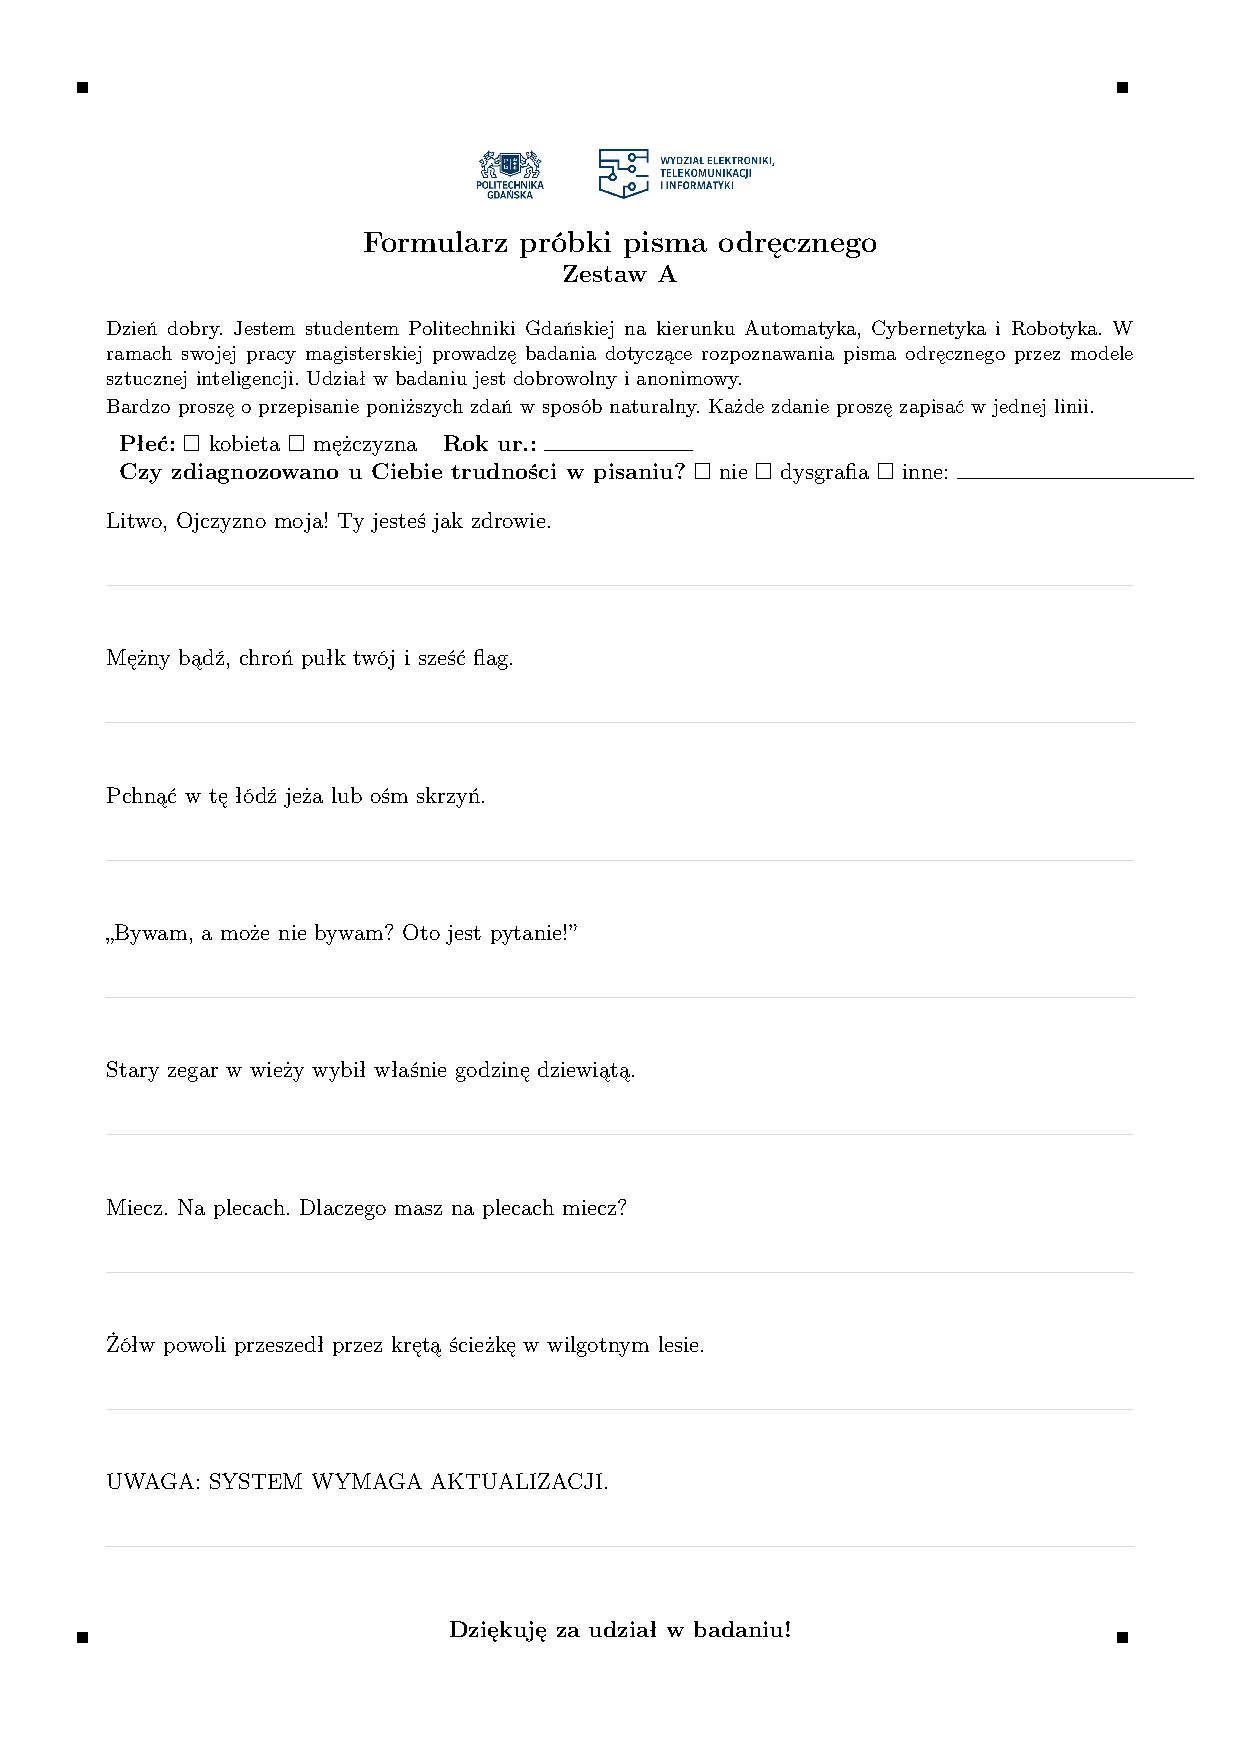
\includegraphics[page=1,width=\textwidth]{Formularze/Formularz.pdf}
        \vspace{2pt}

        {\small Zestaw A}
    \end{minipage}
    \hfill
    \begin{minipage}{0.47\textwidth}
        \centering
        \includegraphics[page=2,width=\textwidth]{Formularze/Formularz.pdf}
        \vspace{2pt}

        {\small Zestaw B}
    \end{minipage}

    \vspace{8pt}

    \begin{minipage}{0.47\textwidth}
        \centering
        \includegraphics[page=3,width=\textwidth]{Formularze/Formularz.pdf}
        \vspace{2pt}

        {\small Zestaw C}
    \end{minipage}
    \caption{Puste formularze użyte do zbierania danych. Każdy wariant zawiera te same pola metadanych oraz osiem linii z tekstami do przepisania.}
    \label{fig:wlasny_zbior_formularze_puste}
\end{figure}

Na formularzach umieściłem czarne kwadratowe znaczniki w rogach strony. Nie były one częścią treści formularza. Służyły do późniejszego wyznaczania położenia kartki na zdjęciu lub skanie. Dzięki nim można było łatwiej sprowadzić różne zdjęcia formularzy do wspólnego układu.

Łącznie zebrałem 320 formularzy. Każdy formularz mógł dostarczyć maksymalnie osiem obrazów linii tekstu. Daje to 2560 możliwych pól z pismem. Część pól była jednak pusta albo nie nadawała się do dalszego użycia. Po sprawdzeniu danych w zbiorze pozostało 2313 obrazów linii.

Uczestników podzieliłem według deklarowanej grupy trudności. Największą część zbioru stanowią osoby bez zadeklarowanych trudności w pisaniu. Druga ważna grupa to osoby z dysgrafią. Pozostałe osoby trafiły do grupy innych trudności.

\begin{table}[H]
    \centering
    \caption{Liczba uczestników i obrazów linii w poszczególnych grupach trudności.}
    \label{tab:wlasny_zbior_grupy}
    \begin{tabular}{lrr}
        \hline
        Grupa & Liczba uczestników & Liczba obrazów linii \\
        \hline
        Brak trudności & 212 & 1594 \\
        Dysgrafia & 71 & 458 \\
        Inne trudności & 37 & 261 \\
        \hline
        Razem & 320 & 2313 \\
        \hline
    \end{tabular}
\end{table}

W grupie innych trudności znalazły się różne deklaracje. Największą część tej grupy stanowiły osoby z dysleksją. W danych znalazły się także dwa przypadki dysortografii. W analizie wyników główną grupą porównawczą pozostaje jednak dysgrafia, ponieważ to ona jest najważniejsza dla celu pracy.

\begin{figure}[H]
    \centering
    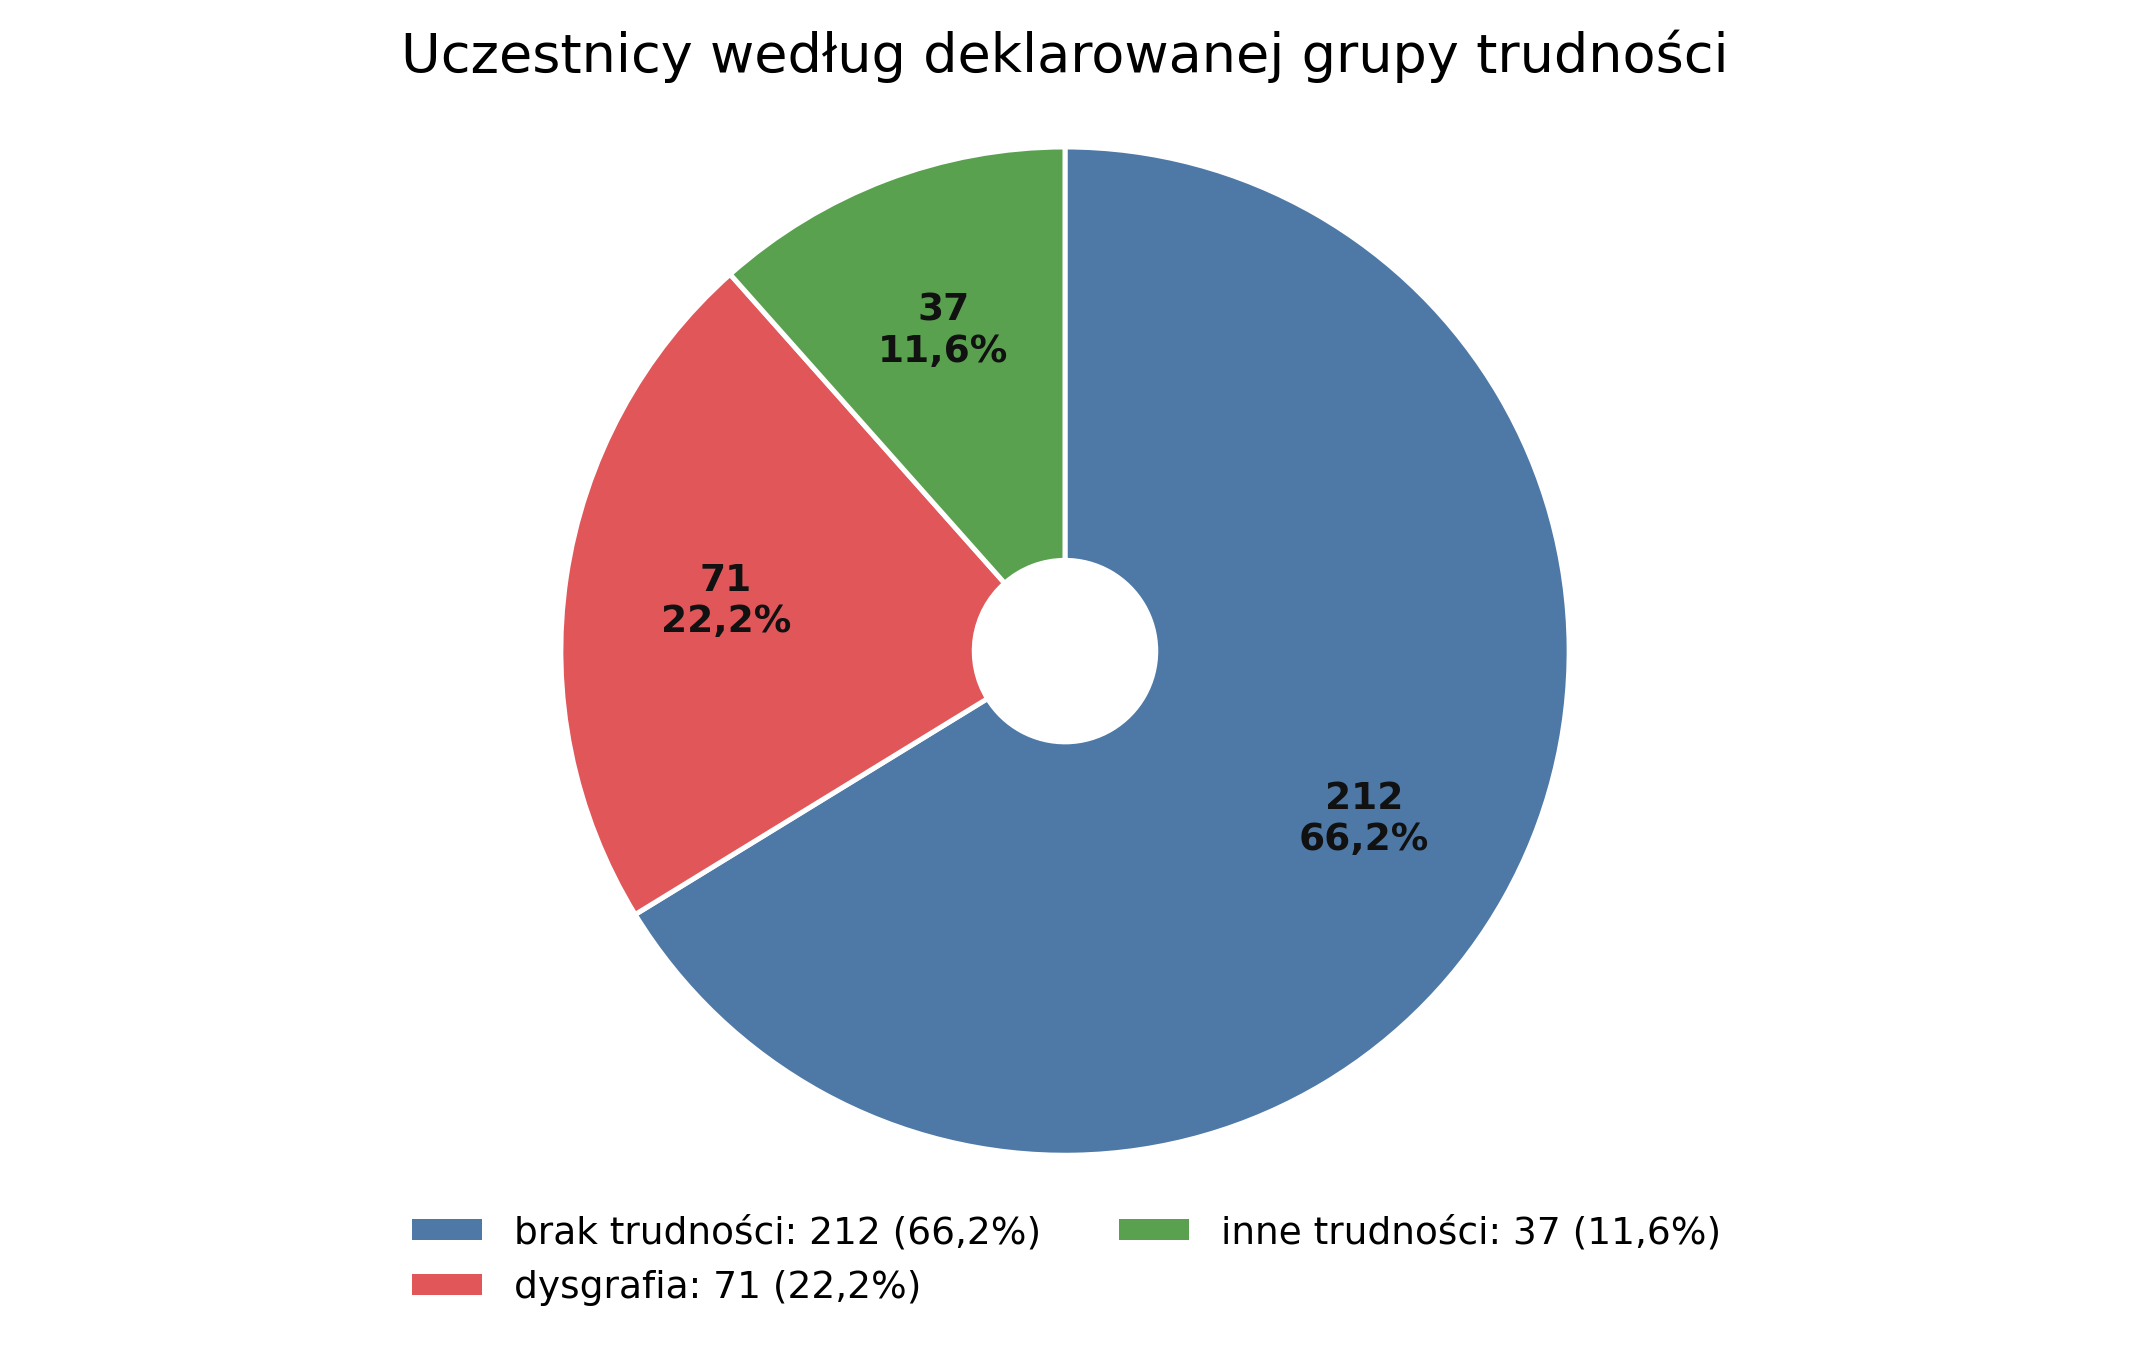
\includegraphics[width=0.82\textwidth]{Formularze/processed_320_check/stats_thesis/figures/uczestnicy_grupa_trudnosci_kolowy.png}
    \caption{Podział uczestników według deklarowanej grupy trudności. Większość osób nie zadeklarowała trudności w pisaniu, ale zbiór zawiera także wyraźną grupę osób z dysgrafią.}
    \label{fig:wlasny_zbior_grupy_kolowy}
\end{figure}

W zbiorze znalazło się 202 mężczyzn oraz 116 kobiet. Dwa formularze miały niejednoznaczne albo nieuzupełnione pole płci, dlatego nie uwzględniłem ich na wykresie płci. Taki zapis pozwala czytelnie pokazać strukturę głównej części zbioru.

\begin{figure}[H]
    \centering
    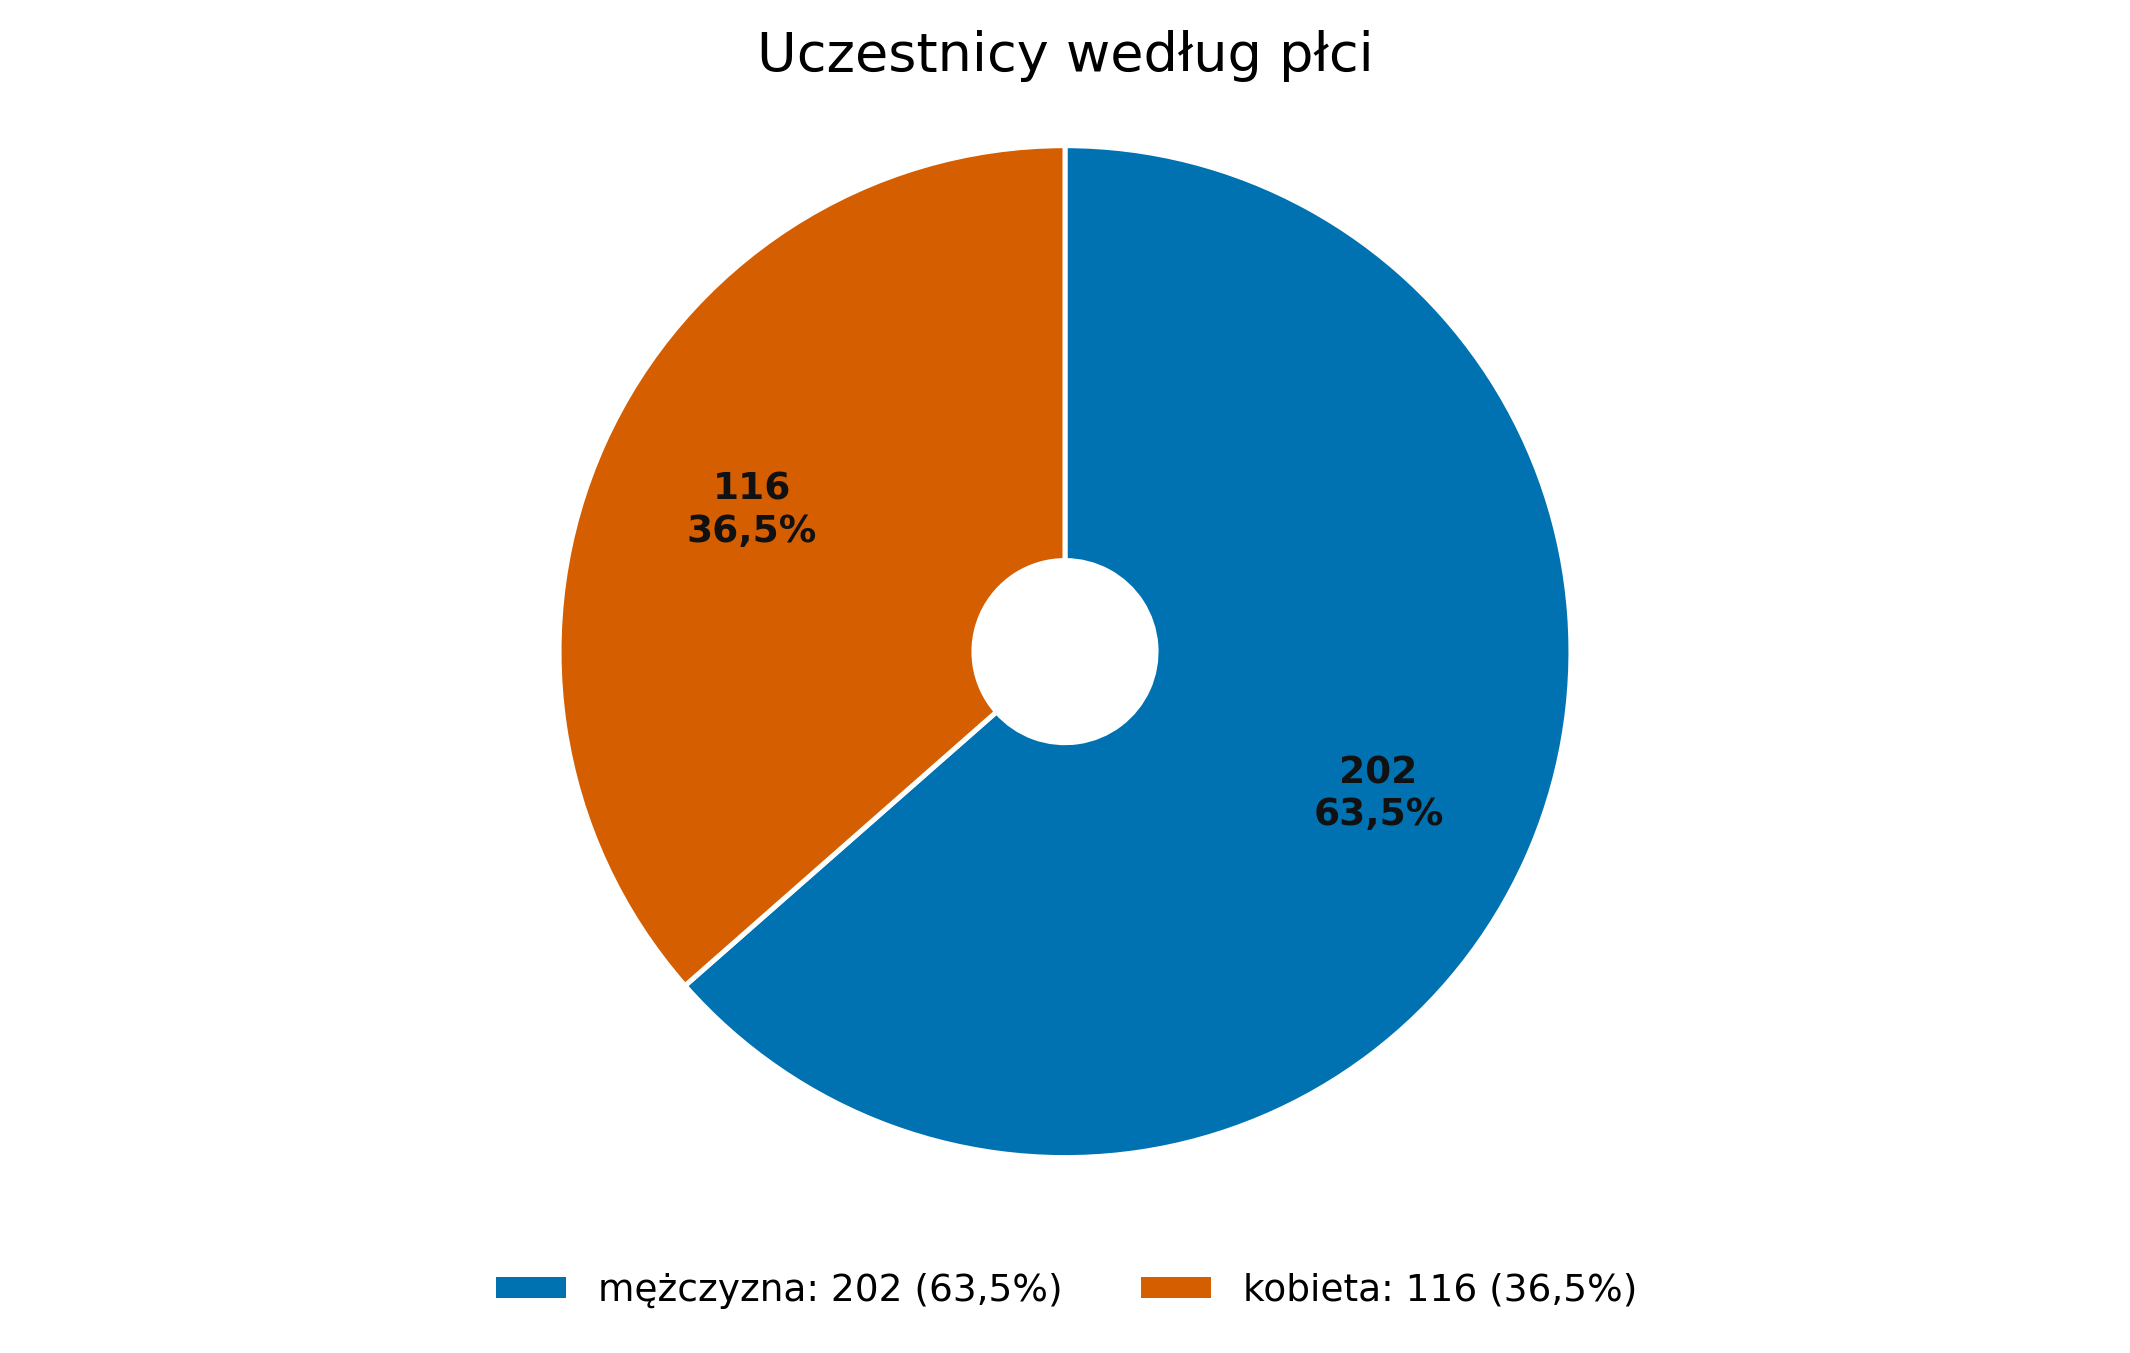
\includegraphics[width=0.78\textwidth]{Formularze/processed_320_check/stats_thesis/figures/uczestnicy_plec_kolowy.png}
    \caption{Podział uczestników według płci po pominięciu dwóch formularzy z nieokreśloną płcią. W zbiorze przeważają mężczyźni.}
    \label{fig:wlasny_zbior_plec_kolowy}
\end{figure}

Uczestnicy pochodzili głównie z roczników 2005--2014. Wiek rocznikowy obliczyłem względem roku 2026. Najliczniejsze były osoby w wieku rocznikowym 16 oraz 17 lat. Rozkład wieku nie jest równomierny, ponieważ dane zbierałem w konkretnych szkołach i klasach.

\begin{figure}[H]
    \centering
    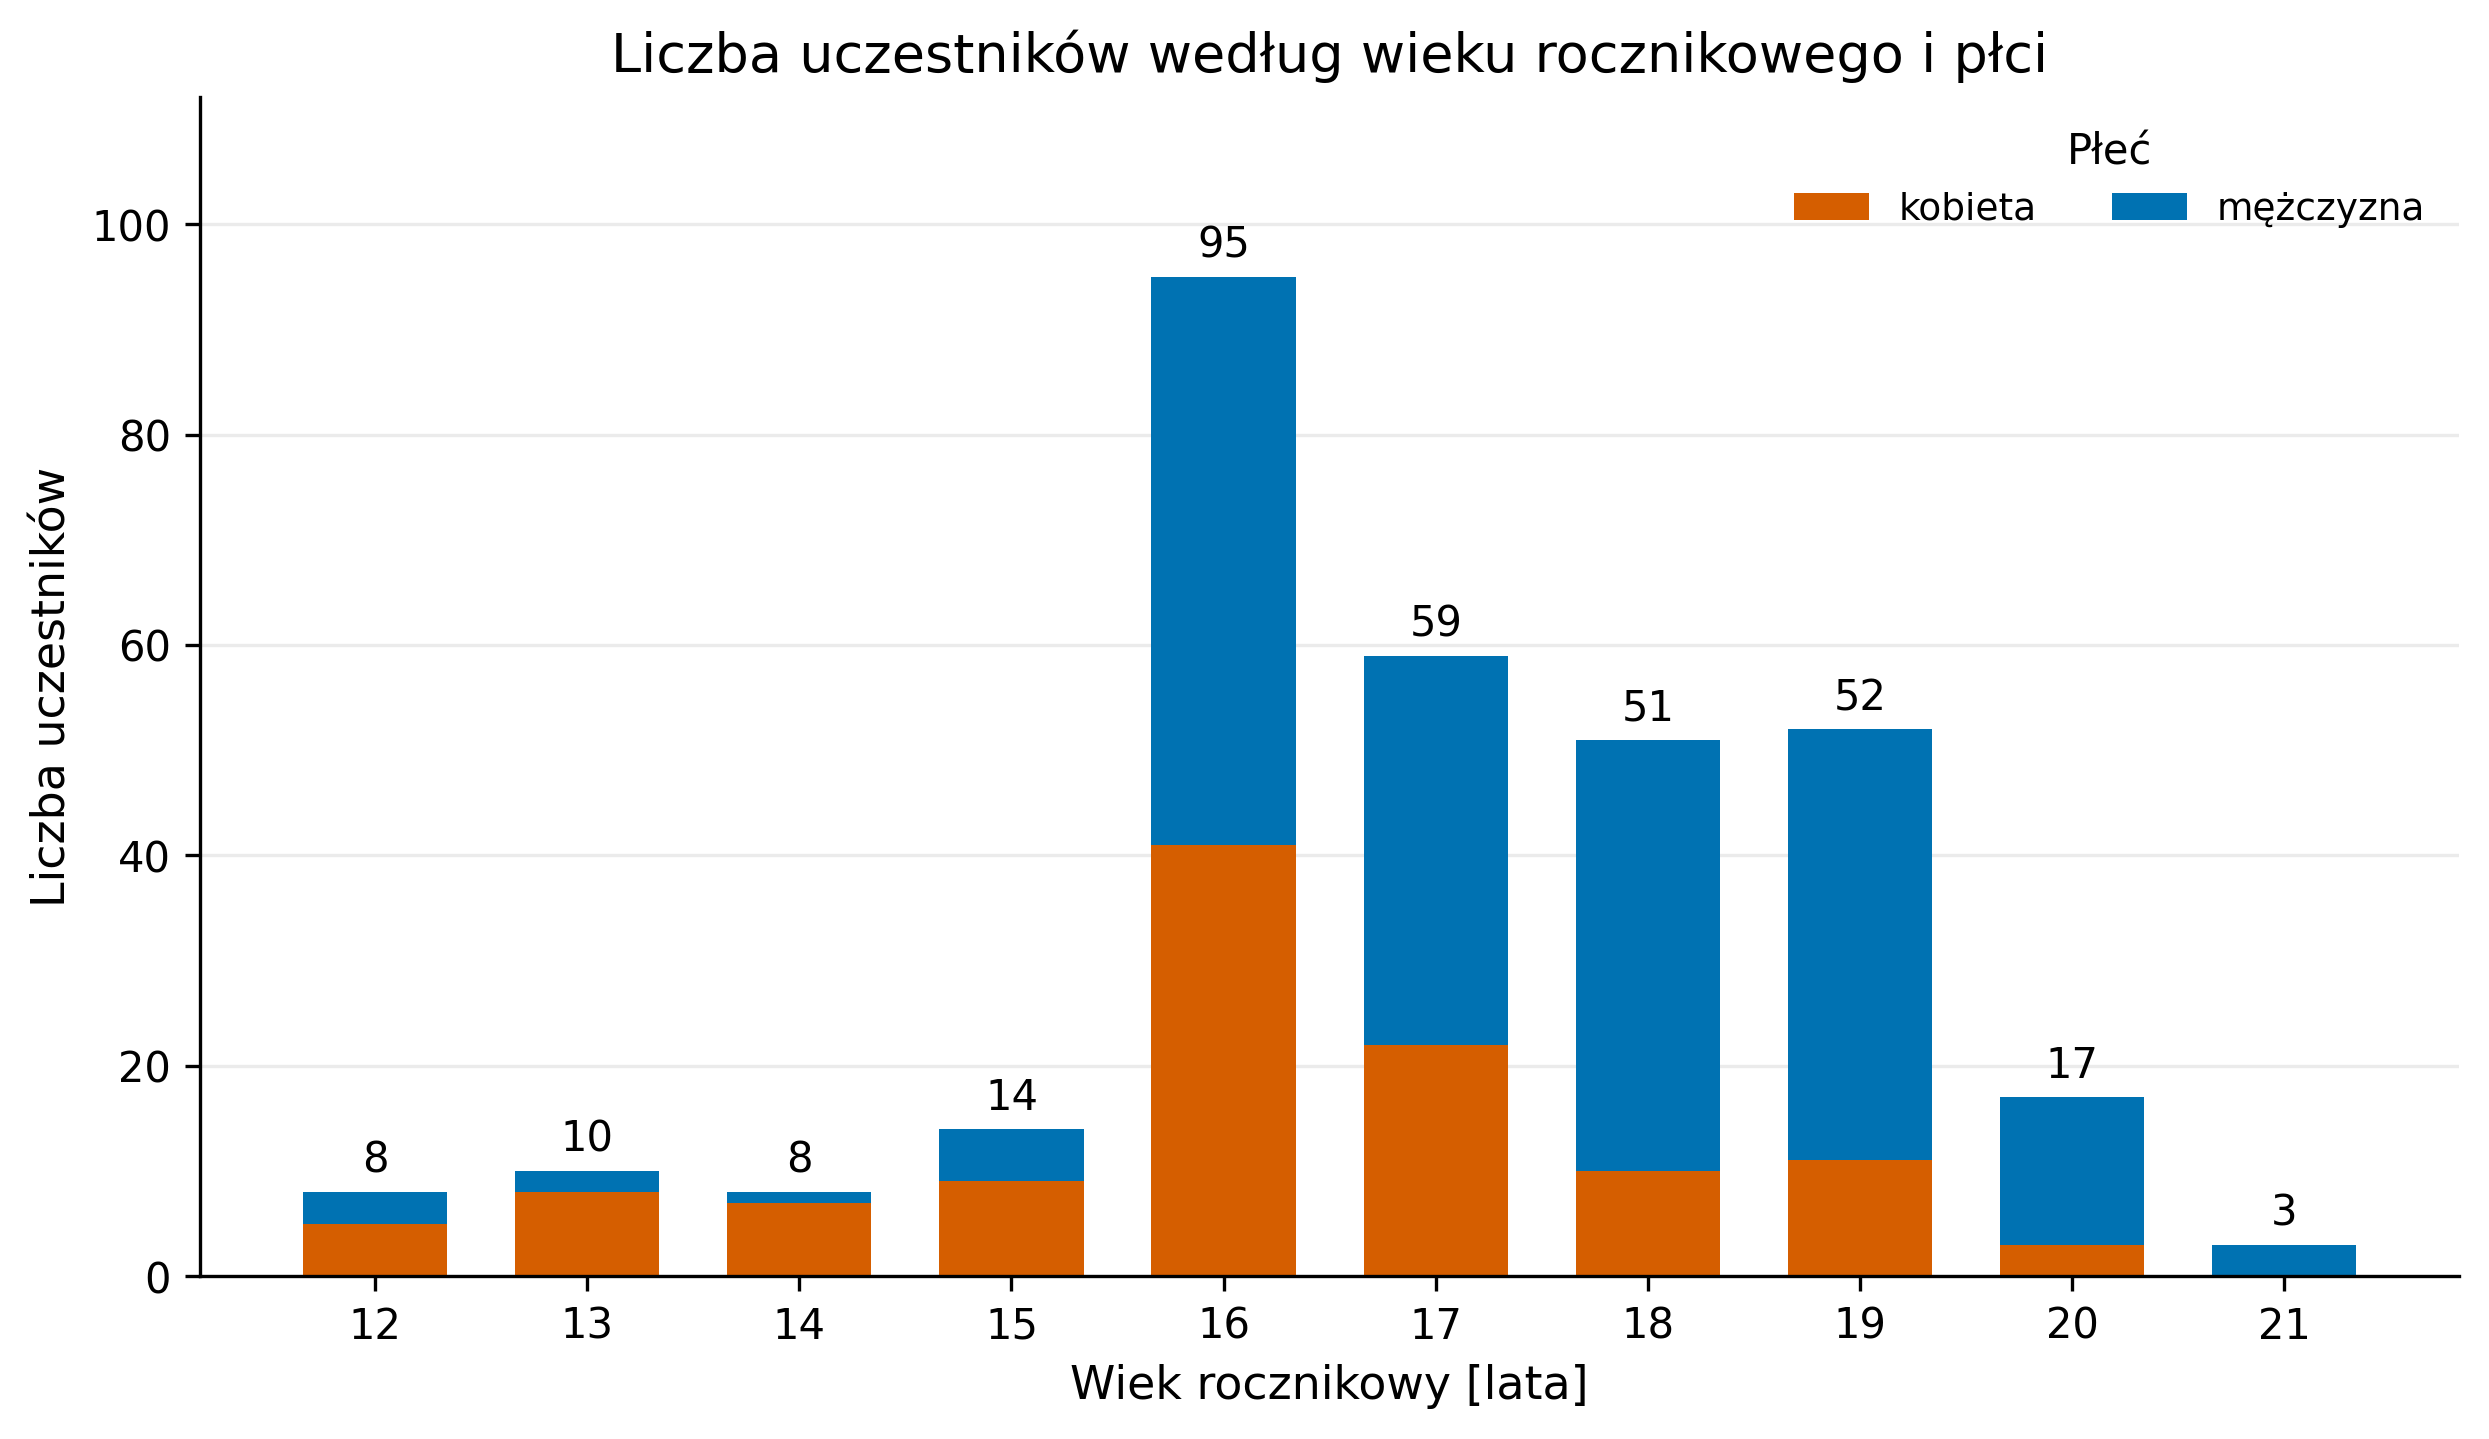
\includegraphics[width=0.95\textwidth]{Formularze/processed_320_check/stats_thesis/figures/uczestnicy_wiek_rocznikowy_plec.png}
    \caption{Liczba uczestników według wieku rocznikowego i płci. Wykres pokazuje, że największą część zbioru stanowią osoby w wieku rocznikowym 16--19 lat.}
    \label{fig:wlasny_zbior_wiek_plec}
\end{figure}

Końcowy zbiór ma strukturę liniową. Oznacza to, że pojedynczą próbką dla modelu jest obraz jednej linii tekstu oraz odpowiadająca mu transkrypcja. Taki format pasuje do modeli rozpoznawania pisma odręcznego, które zwykle uczą się na wycinkach zawierających pojedyncze linie.

\begin{figure}[H]
    \centering
    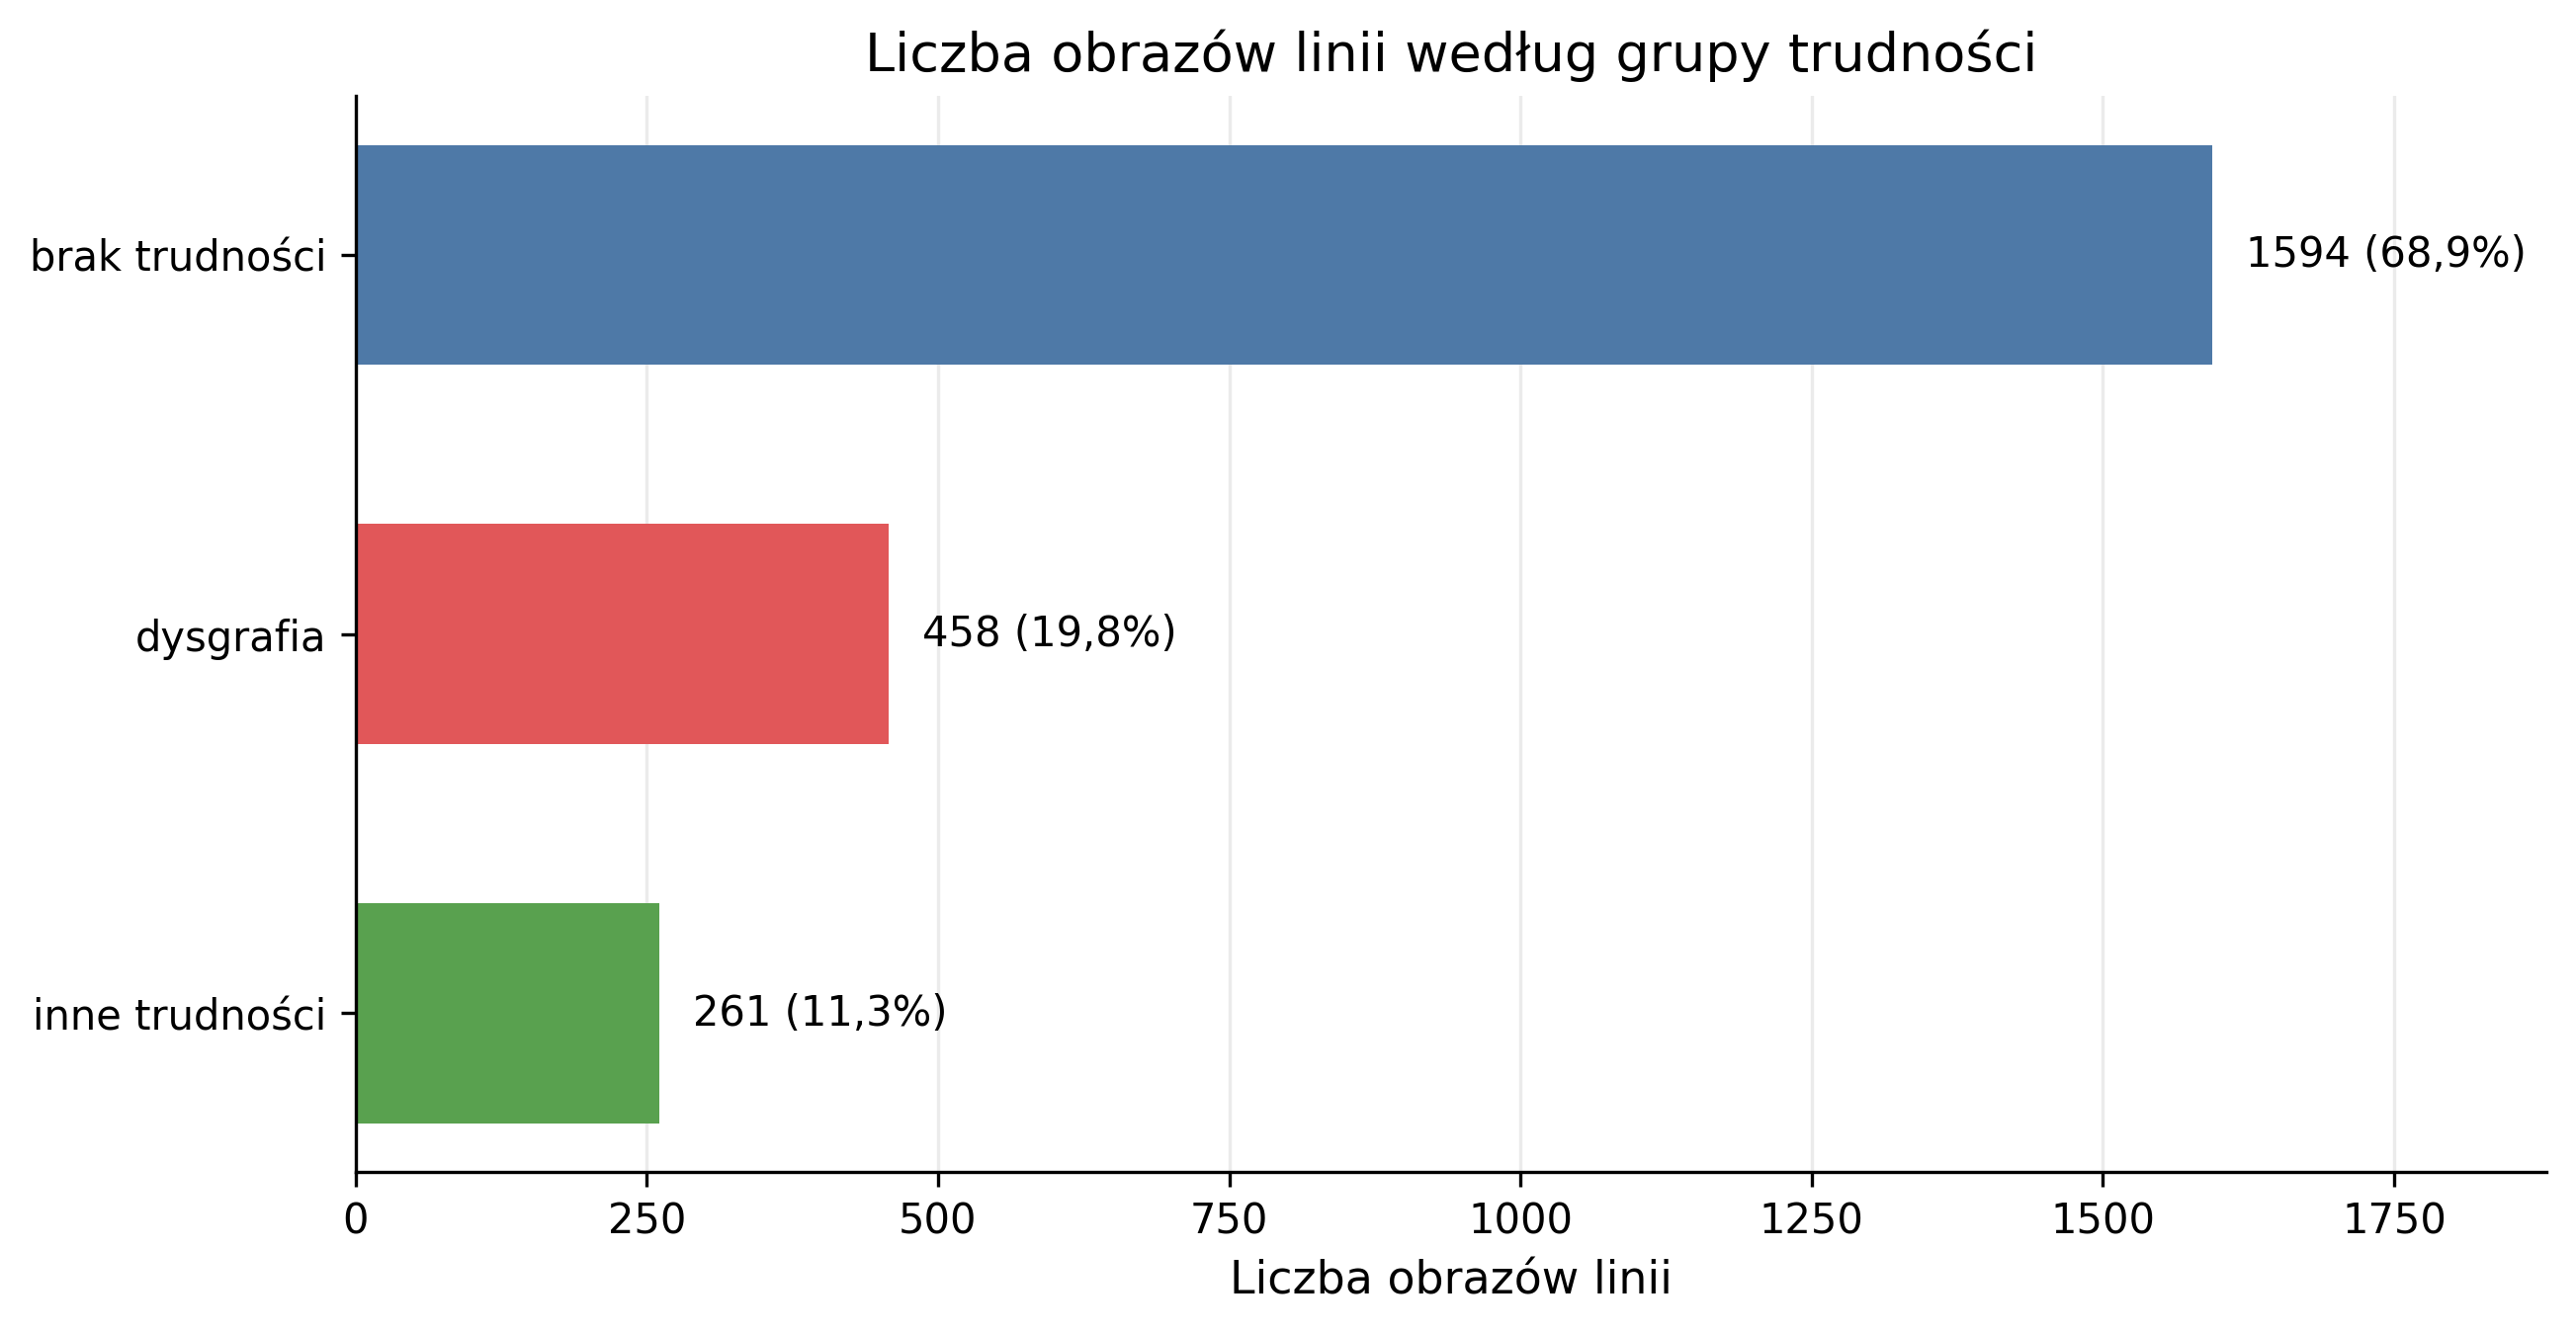
\includegraphics[width=0.9\textwidth]{Formularze/processed_320_check/stats_thesis/figures/obrazy_linii_grupa_trudnosci_pl.png}
    \caption{Liczba obrazów linii w finalnym zbiorze według grupy trudności. Najwięcej próbek pochodzi od osób bez zadeklarowanych trudności, ale zbiór zawiera także osobną część z pismem dysgraficznym.}
    \label{fig:wlasny_zbior_linie_grupy}
\end{figure}

Zbiór podzieliłem na część treningową, walidacyjną i testową. Podział wykonałem na poziomie uczestnika. Dzięki temu linie zapisane przez tę samą osobę nie trafiają jednocześnie do różnych części zbioru. Ogranicza to ryzyko zawyżenia wyników podczas ewaluacji.

\begin{table}[H]
    \centering
    \caption{Podział finalnych obrazów linii na zbiory treningowy, walidacyjny i testowy.}
    \label{tab:wlasny_zbior_split}
    \begin{tabular}{lr}
        \hline
        Część zbioru & Liczba obrazów linii \\
        \hline
        Treningowa & 1844 \\
        Walidacyjna & 228 \\
        Testowa & 241 \\
        \hline
        Razem & 2313 \\
        \hline
    \end{tabular}
\end{table}

Tak przygotowany zbiór pozwala porównać modele w kilku warunkach. Można analizować wyniki dla całego zbioru, dla osób bez trudności oraz dla osób z dysgrafią. Można także sprawdzić, czy dostrojenie modelu poprawia rozpoznawanie tekstu pisanego przez osoby z trudnościami w pisaniu.

\FloatBarrier
